\section{Background}
\label{section:background}

Heating, ventilation and air conditioning (\gls{hvac}) is a technology of indoor environmental comfort. It is usually implemented in large office, commercial and industrial buildings such as schools, airports, malls, factories, hospitals, etc. Its ultimate goal is to maintain thermal comfort and create healthy indoor air quality while keeping an affordable maintenance cost, being energy efficient and environmentally friendly.

Currently, \gls{hvac} is comprised of numerous components, advanced sensing technologies, advanced control algorithms and even artificial intelligence techniques, which have been introduced to help the system meet its operational objectives across different types of buildings worldwide. Hence \gls{hvac} systems are regarded as highly interdisciplinary and complex mechanical systems.

According to the U.S. Energy Information Administration, residential and commercial sectors account for $40\%$ of the total share of energy consumed in the United States in 2016 \cite{us_energy_usage}. Heating, ventilation and air conditioning make up almost $50\%$ of the total energy consumption \cite{residential_energy_use_us, commericial_energy_use_us}.

As with any other mechanical system, \gls{hvac} systems are prone to faults and as its scale and complexity increases the detection, identification and pinpointing of such faults within the \gls{hvac} network becomes a very challenging and hard to achieve task. Here, faults include not only complete equipment failures, but also non-optimal operating conditions, e.g., occupant discomfort, energy inefficiency, poor choice of operating targets, sensor calibration error, poor controller tuning, etc. Some common faults that an \gls{hvac} system may be prone to are: a stuck damper, stuck water valve, coolant leakage, airflow leakage (due to breaches in the ducts), fan malfunction, etc. Such failures may degrade the overall performance of the \gls{hvac} system and thus lead to energy waste. Therefore, it is of great potential to develop automatic, quick responding, intelligent, and reliable monitoring and diagnosis tools to ensure the normal operation of the system, increasing, as a direct consequence, its energy consumption efficiency.

According to the National Institute of Standards and Technology (\gls{nist}), Fault Detection and Diagnosis (\gls{fdd}) methods have a potential to save 10\%-40\% of \gls{hvac} energy consumption \cite{schein1}. \gls{fdd} tools for \gls{hvac} is therefore critical to increase the energy efficiency for buildings. Since the 1980s, researchers have been striving to improve the energy efficiency of the system due to rising energy costs and increased awareness of the environment.

\subsection{Fault Detection in \gls{hvac} systems}

As mentioned in the previous section, \gls{fdd} tools can help improve the overall energy consumption of and \gls{hvac} system by timely detecting, isolating (classifying) and pinpointing the location of the faults so that they can be fixed as soon as they are detected. Several methods have been proposed for achieving this goal. 

Fault Detection and Isolation (\gls{fdi}) is a subfield of control engineering concerned with monitoring a system, identifying when a fault has occurred, and pinpointing the type of fault and its location. Usually the methods and techniques for doing \gls{fdi} can be divided in two groups:

\begin{itemize}
\item A model based approach that measures the discrepancies between the actual sensor readings and the expected values derived from the model.
\item A pattern recognition approach that looks for patterns in the data that may indicate a fault.
\end{itemize}

In the first group some model of the system is used to decide about the occurrence of a fault. The model may be mathematical or knowledge based, here energy and thermal models have been used to successfully identify certain faults and tune the controllers as in \cite{wu_thesis, wei_thesis, model_fault_detection1}. In the second group some mathematical or statistical operations are performed to the measurements, this approach also considers machine learning algorithms that will look for patterns in the data which may be indicative of a fault. Such approaches have been specially considered in the domain of machine learning as in \cite{fault_detection_mechanical1, fault_diagnosis_ahu, cmeans_fault_detection, fault_diagnosis_refrigerant}.

In this work the pattern recognition approach is considered over the model based one, this will allow the system to detect, classify and locate faults within the system without specific knowledge of the network except for its topology.

\subsection{A generic \gls{hvac} system}

A generic \gls{hvac} is comprised of several components, among the most noticeable ones we can find are: the Air Handling Unit, the Variable Air Volume, the Staged Air Volume and the Thermafuser.  The Air Handling Unit (\gls{ahu}) is the main component of the \gls{hvac} network. The function of the \gls{ahu} is to regulate, condition and distribute the conditioned air to the other components of the system though  a ductwork ventilation system which is also used for returning air to the \gls{ahu}. \gls{ahu} is usually a large metal box containing inside fans, heating and/or cooling elements, filter racks or chambers, sound atenuators and dampers. Figure \ref{fig:ahu_inside} shows an inside view of how the majority of \gls{ahu}s are built, while Figure \ref{fig:ahu_inside} shows and outside view of an \gls{ahu}.

\begin{figure}[H]
	\centering
		\begin{minipage}{.5\textwidth}
 			 \centering
  			\includegraphics[width=55mm, height=45mm]{resources/AHUInside.png}
  			\caption{Inside view of \gls{ahu}}
  			%\captionof{figure}{A figure}
 			 \label{fig:ahu_inside}
		\end{minipage}%
		\begin{minipage}{.5\textwidth}
  			\centering
  			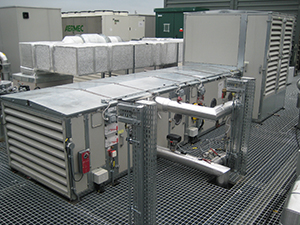
\includegraphics[width=55mm, height=45mm]{resources/AHUOutside.png}
  			\caption{Outside view of \gls{ahu}}
  			%\captionof{figure}{Another figure}
  			\label{fig:ahu_outside}
		\end{minipage}
\end{figure}

In the second level of the \gls{hvac} topology we have the Variable Air Volume (\gls{vav}) and the Staged Air Volume (\gls{sav}). The main goal of these two components is two vary the airflow and the temperature of the supply air to be further distributed, they achieve this goal by controlling the damper position at the entrance of the \gls{vav}/\gls{sav} and modifying the temperature by means of cooling and heating coils. Figure ... shows the inside composition of a generic \gls{vav} while Figure ... shows the inside composition for a generic \gls{sav}.

\begin{figure}[H]
	\centering
		\begin{minipage}{.5\textwidth}
 			 \centering
  			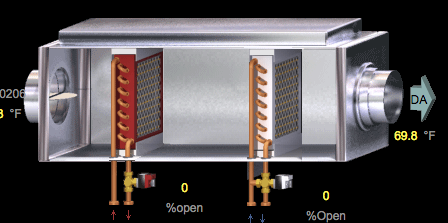
\includegraphics[width=55mm, height=45mm]{resources/VAVInside.png}
  			\caption{Inside view of a \gls{vav}}
  			%\captionof{figure}{A figure}
 			 \label{fig:vav_inside}
		\end{minipage}%
		\begin{minipage}{.5\textwidth}
  			\centering
  			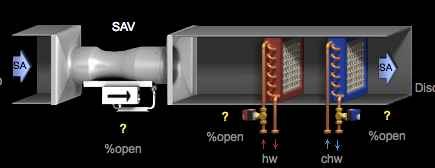
\includegraphics[width=55mm, height=45mm]{resources/SAVInside.png}
  			\caption{Outside view of a \gls{sav}}
  			%\captionof{figure}{Another figure}
  			\label{fig:sav_inside}
		\end{minipage}
\end{figure}

Finally, the last component in the chain are the Thermafusers, these components are where the air comes out into the room and their purpose is to regulate the airflow that comes into the room, it achieves this goal by using a set of dampers along its edges. Figure \ref{fig:thermafuser} shows a generic thermafuser mounted on the ceiling of a room.

\begin{figure}[H]
	\centering
  	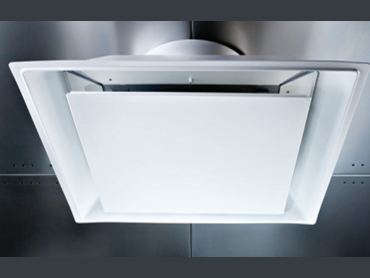
\includegraphics[width=55mm, height=45mm]{resources/thermafuser.png}
  	\caption{View of a thermafuser}
  	%\captionof{figure}{A figure}
 	\label{fig:thermafuser}
\end{figure}

Although a description of the top-down air supply chain is given here, it is important to emphasize that some of the air used in the rooms goes back into the system for its reuse by means of return air grilles on the roof of the rooms, which travels all its way back to the \gls{ahu} where some of it is reused.

Finally, it is worth to mention that the \gls{hvac} system of SE 2 is comprised by 4 \gls{ahu}, about 150 \glspl{vav}/\glspl{sav} and  about 150 thermafusers.